\documentclass[12pt]{article}
\usepackage{fullpage}
\usepackage{amsmath, amsthm, amssymb}
\usepackage{enumerate}
\usepackage{mathtools}
\usepackage{multicol}
\usepackage{nicefrac}
\usepackage{graphicx}
\usepackage{hyperref}

\usepackage{tikz}
\usetikzlibrary{calc}
\usetikzlibrary{backgrounds}
\usepgflibrary{shapes}
\usetikzlibrary{through}

\usepackage{float}
\newtheorem{lemma}{Lemma}
\newtheorem{theorem}{Theorem}
\newtheorem{claim}{claim}
\newtheorem*{lemma*}{Lemma}
\newtheorem*{theorem*}{Theorem}
\newtheorem*{claim*}{Claim}
\usepackage{subcaption}

\newcommand*{\Real}{\mathbb{R}}
\newcommand*{\Z}{\mathbb{Z}}
\newcommand*{\Q}{\mathbb{Q}}
\newcommand*{\F}{\mathbb{F}}
\newcommand*{\ord}{\mathrm{ord}}
\newcommand*{\nil}{\mathfrak{N}}
\newcommand*{\inv}{^{-1}}

\begin{document}

\title{MATH 4320 Homework 5}
\author{Dominick Twitty}
\date{}
\maketitle

\section{On Algebraic Elements of an Extension}
%TODO 1
\begin{claim*}
Let $F$ be a field and $K$ be an extension. If $\alpha, \beta \in K$ are algebraic, then $\alpha \pm \beta$, $\alpha \beta$, and $\nicefrac{\alpha}{\beta}$ are also algebraic.
\end{claim*}
\begin{proof}
Let $a \in F[x]$ with degree $m$ be the minimum polynomial such that $a(\alpha) = 0$. Let $b$ with degree $m$ be a similar polynomial for $\beta$. Then $[F(\alpha) : F] = n$ and $[F(\beta) : F] = m$. We can say that $[F(\alpha, \beta) : F(\alpha)]$ is at most $m$ and is therefore finite. By the multiplicity formula for degrees, $[F(\alpha,\beta) : F]$ is at most $nm$, and is therefore finite. Furthermore, $F(\alpha, \beta)$ is a field, meaning $F(\alpha, \beta)$ contains $\alpha \pm \beta$, $\alpha \beta$, and $\nicefrac{\alpha}{\beta} = \alpha \beta\inv$. Finally, by Corollary 3.117 in the textbook, all of the listed elements are the roots of a monic irreducible polynomial in $F[x]$ and are therefore algebraic.
\end{proof}



\section{On Nilpotents and Ideals}
\begin{claim*}
$\nil(R)$ is ideal in $R$.
\end{claim*}
\begin{proof}
First, we show that $\nil(R)$ is a group under addition. Clearly, $0$ is in $\nil(R)$. Next, for some $x,y \in R$, let $x^n = y^m = 0$. We see
\[ (x + y) ^ {m + n - 1} = \sum_{k = 0}^{m + n - 1} \binom{n}{k} x^{m + n - 1 - k} y^k = 0\]
Finally, let $x ^ m = 0$. If $m$ is even, then $(-x) ^ m = x ^ m = 0$. If $m$ is odd, then $(-x) ^ {m + 1} = (-x)(-x)^m = 0$. Then $\nil(R)$ is a group under addition. Next, we must show that $\nil(R)$ absorbs multiplications. Let $x^m = 0$, and $y \in R$. Then
\[ (xy) ^ m = x^m y^m = 0 \]
So, $\nil(R)$ is an ideal. An alternative proof is that $\nil(R) = \sqrt{\{0_R\}}$. We see that $\{0_R\}$ is an ideal, and we showed in a previous homework that radical of an ideal is an ideal.
\end{proof}

\begin{claim*}
$R/\nil(R)$ has only $0$ as a nilpotent element.
\end{claim*}
\begin{proof}
Let $(x + \nil(R)) ^ m = (0 + \nil(R))$. Then $(x + \nil(R))^m = (x ^ m + \nil(R)) = 0 + \nil(R)$.
Then, $x^m \in \nil(R)$, and $x \in \nil(R)$. Finally, $(x + \nil(R)) = (0 + \nil(R))$. 
\end{proof}


\section{On Polynomial Quotient Fields}
Let $f = x^2  + x + 1 \in \F_2[x]$. Let $I = (f)$, and $E = \F_2[x] / I$. By Theorem 3.115 in the textbook, we can say that every $e \in E$ has a unique expression of the form $a + b(x + I)$ where $a,b \in \F_2$ and $(x + I)$ is a root of $f$. There are four choices of $(a, b)$, so $E = \{0 + I, 1, x + I, 1 + x + I\}$. As shown in the proof of Theorem 3.115, by the division algorithm, if $g = qf + r$, then $g + I = r + I$. This gives us the following three equations
\begin{align*}
(x)(x) = x^2 = f + x + 1 &\implies (x + I)(x + I) = (x + 1 + I)\\
(x)(x + 1) = x^2 + x = f + 1 &\implies (x + I)(x + 1 + I) = (1 + I)\\
(x + 1)(x + 1) = x^2 + 1 = f + x &\implies (x + 1 + I)(x + 1 + I) = (x + I)
\end{align*}
\noindent and the multiplication table
\[
\begin{array}{c | c c c c}
      & 0 & 1 & x& x + 1\\\hline
0     & 0 & 0     & 0     & 0\\
1     & 0 & 1     & x     & x + 1\\
x     & 0 & x     & x + 1 & 1\\
x + 1 & 0 & x + 1 & 1     & x
\end{array}
\]
Every nonzero element of $E$ has an inverse, then $E$ is a field, then $f$ is irreducible.

\section{On $x^3 - 2x - 2$ in $\Q[x]$}
Let $f = x^3 - 2x - 2 \in \Q[x]$. We see that $f$ meets the Eisenstein Criterion with prime $p = 2$, and is therefore irreducible over $\Q$. Let $\theta$ be a root of $f$. We see that 
\begin{align*}
(3 + \theta)(5 \theta^2 -2\theta + 10) &= 5\theta^3 + 13 \theta^2 + 4\theta + 30\\
&= 5f(\theta) + 13\theta^2 + 14\theta + 40\\
&= 13\theta^2 + 14\theta + 40
\end{align*}

Let $g = 5\theta^2 - 2\theta + 10$. We wish to find some $h$ such that $hg = 1 \equiv qf + 1$. Given that $f$ and $g$ are relatively prime ($f$ is irreducible and does not divide $g$), we can find $h$ and $q$ using the Extended Euclidean Algorithm. With the help of a computer algebra system, we find that $\frac{1}{h} = g$ with
\begin{align*}
g = \frac{-96 \theta^2 + 70\theta + 412}{5204} 
&& \text{and} && 
gh = \left(\frac{-120\theta}{1301} + \frac{271}{2602}\right)f + 1
\end{align*}


\section{}
%TODO 5
\begin{claim*}
Let $F$ be a field with characteristic $\neq 2$. Let $D_1, D_2 \in F$ not be squares. $F(\sqrt{D_1}, \sqrt{D_2})$ is a degree 4 extension if $D_1D_2$ is not square in $F$, else degree 2
\end{claim*}

\begin{proof}
First, we see that $F(\sqrt{D_1})$ is a degree 2 extension. We can see this by constructing $p = x^2 - D_1 \in F[x]$, which has $\sqrt{D_1}$ as a root. AS $p$ has degree two, and $\sqrt{D_1} \notin F$, $p$ is irreducible, and $F[x] / (p) = F(\sqrt{D_1})$ has degree 2. Similar thinking holds for $F(\sqrt{D_2})$.

Treating $F(\sqrt{D_1}, \sqrt{D_2})$ as $F(\sqrt{D_1})(\sqrt{D_2})$, all elements have the form
\begin{align*}
(a + b\sqrt{D_1}) + (c + d\sqrt{D_1})\sqrt{D_2}\\
a + b\sqrt{D_1} + c\sqrt{D_2} + d\sqrt{D_1 D_2}
\end{align*}
with $a,b,c,d \in F$. If $\sqrt{D_1 D_2} \notin F$, then we have a vector space of size 4. However, if $\sqrt{D_1 D_2} \in F$, then $d\sqrt{D_1 D_2} \in F$, and we have at most a vector space of size 3. 
\end{proof}



\section{On the Equality of Field Extensions}
\begin{claim*}
$\Q(\sqrt{2} + \sqrt{3}) = \Q(\sqrt{2}, \sqrt{3})$
\end{claim*}
\begin{proof}
First, we see that because both $\sqrt{2}$ and $\sqrt{3}$ have degree 2 in $\Q$, then
\[\Q(\sqrt{2}, \sqrt{3}) = \{a + b\sqrt{2} + c\sqrt{3} + d\sqrt{6} \, | \, a,b,c,d \in \Q\}\]
Clearly $\Q(\sqrt{2} + \sqrt{3}) \subseteq \Q(\sqrt{2}, \sqrt{3})$. As $\Q(\sqrt{2} + \sqrt{3})$ is a field, it must contain inverses. Then
\[(\sqrt{2} + \sqrt{3})\inv = \frac{1}{\sqrt{2} + \sqrt{3}} = \frac{\sqrt{2} - \sqrt{3}}{2 - 3} = \sqrt{3} - \sqrt{2} \in \Q(\sqrt{2} + \sqrt{3})\]
From this, $\Q(\sqrt{2} + \sqrt{3})$ contains both $\sqrt{2}$ and $\sqrt{3}$. Then $\Q(\sqrt{2}, \sqrt{3}) or \subseteq \Q(\sqrt{2} + \sqrt{3})$
\end{proof}
\noindent Let $z = \sqrt{2} + \sqrt{3}$. We construct an irreducible polynomial $p$ with $p(z) = 0$
\begin{align*}
z &= \sqrt{2} + \sqrt{3}\\
z^2 &= 5 + 2 \sqrt{6}\\
(z^2 - 5)^2 &= 24\\
z^4 - 10z^2 + 1 &= 0
\end{align*}
So $p = x^4 - 10x^2 + 1$

\section{On the Non-Constrctability of a Regular Heptagon}
By Theorem 4.59 in the textbook, a $p$-gon for prime $p$ is constructible if and only $p = 2 ^ {2 ^ k} + 1$ for some $k$. These numbers, called the Fermat Primes, include $3, 5, 17, 257, \ldots$, but not $7$. Therefore, it is impossible to construct a regular heptagon with straightedge and compass.


\section{Inscribing a Hexagon in a Circle}
Consider some regular hexagon $H$ inscribed in a circle $C$ with center $o$ and radius $r$. Let $p_1$ and $p_2$ be adjacent vertices of $H$. We see that the triangle $(p_1,p_2,o)$ is equilateral. From this, we can say that the side length of $H$ is exactly equal to $r$.

\begin{figure}[H] \centering
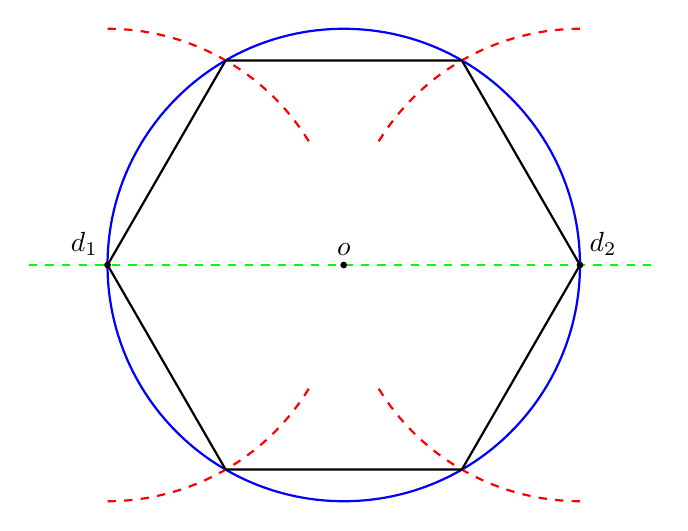
\begin{tikzpicture}
    % the circle
    \draw[thick, blue] (6*2,0) circle(3cm);
    
    % the center line
    \draw[thick,green,dashed] (8,0) -- (16,0);
    
    % the arcs from d1 and d2
    \draw[thick,red,dashed] (9,3) arc (90:30:3);
    \draw[thick,red,dashed] (9,-3) arc (-90:-30:3);
    \draw[thick,red,dashed] (15,3) arc (90:150:3);
    \draw[thick,red,dashed] (15,-3) arc (-90:-150:3);
    
    % the constructed hexagon
    \node[thick, regular polygon, regular polygon sides=6, minimum size=6cm, draw] at (6*2,0) {};
    
    % labelled points
    \draw [fill=black] (12,0) circle (1pt);
    \node[above] at (12,0) {$o$};
    \draw [fill=black] (9,0) circle (1pt);
    \node[above left] at (9,0) {$d_1$};
    \draw [fill=black] (15,0) circle (1pt);
    \node[above right] at (15,0) {$d_2$};
\end{tikzpicture}
\end{figure}

This gives us an easy way to construct $H$, which we illustrate above. Draw a line (shown in green) across $C$, passing through $o$, to find points $d_1$ and $d_2$ exactly opposite each other on $C$. Set the radius of the compass to $r$ by extending it from $d_1$ to $c$. Intersect arcs (shown in red) of radius $r$ centered at $d_1$ with $C$, and do the same with $d_2$. Connect the six points to draw an regular inscribed hexagon.

By construction, each intersection point is distance $r$ from its arc center. We know $d_1$ and $d_2$ can be part of a hexagon, as they are exactly opposite each other. We showed above that the points of distance $r$ away from $d_1$ on $C$ must also be part of the hexagon, so the four intersections are also part of the hexagon. 

\section{On Splitting for Prime Cyclotomic Polynomials}
We wish to show that $\phi_p$ can be decomposed into linear factors in $\Q(\zeta_p)$, where $\zeta_p$ is a $p$th root of unity. To start, we notice that because $p$ is prime, $\Q(\zeta_p)$ contains all $p - 1$ $p$th roots of unity. Notice that $(x - 1)\phi_p = x^p - 1$, which has roots $1, \zeta_p, \zeta_p^2,\ldots,\zeta_p^{p - 1}$. We see that
\[ x ^ p - 1 = \prod_{k = 0}^{p - 1} (x - \zeta_p ^ k) \]
Clearly $x^p - 1$ splits over $\Q(\zeta_p)$, and as a divisor, $\phi_p$ must also split over $\Q(\zeta_p)$.
\section{On Specific Splitting Fields}
We see that $x^4 + x^2 + x + 1$ in $\F_2$ factors into $(x + 1)(x^3 + x^2 + 1)$. We take the root $z$ of the cubic irreducible factor and generate the field $E = \F_2[x] / (x^3 + x^2 + 1) = \F_2(z)$ where $z^3 + z^2 = 1$. After a bit of labor in factoring (by hand this time, no Python script), we have
\[x^4 + x^2 + x + 1 = (x + 1)(x + z)(x + z^2)(x + (1 + z + z^2))\]
We have shown a linear factorization of the polynomial, therefore the splitting field is $\F_2(z)$.

\end{document}
